\documentclass[12pt]{report}
\usepackage{geometry}
\usepackage{graphicx}

\geometry{margin=1in}
\setcounter{tocdepth}{2}

\title{CS328 Final Project - Mechanics}
\date{\today}
\author{Mason Fabel - \textit{fabe0940@vandals.uidaho.edu}}

\begin{document}

\maketitle

\tableofcontents
\clearpage

\chapter{Overview}

This game will be a 2D, two player fighting game featuring graduate students
from different majors competing with each other in order to earn their
department the ``Major of the Year'' award.

The target audience is those who do not regularly play fighting games, so the
focus will be placed on clear and simple to grasp mechanics rather then deep
or competetively viable gameplay.

In keeping with the casual feel of the game, there will not be any computer
controlled opponents. Rather, two humans will be required to play the game.
To facilitate this, the game will be playable over a local area network on
two different computers.

This game will be controlled exclusively by keyboard input, although an optional
Playstation 3 wireless controller will be supported on OSX 10.7.

\chapter{Gameplay}

\begin{section}{Modes}
This game will feature a single mode of play, which is a 1 versus 1 mode where
two human players fight each other, and the first player to knock out their
oppenent twice wins.

This single mode will come in two flavors: Host mode and Join mode. These two
modes will play identically, but will behave differently under the hood.

\begin{subsection}{Host}
The first mode is Host mode. In this mode, a server process is started in
addition to the main game process. This server is then connected to by the game
and can additionally be joined by one one clien in Join mode.

Once the client/server connection is established, the server procees to manage
the actual gameplay, recieving input from the clients and sending enough
information back to the clients to allow them to completely render the current
state of the game.
\end{subsection}

\begin{subsection}{Join}
In addition to Host mode, there is also Join mode. This mode connects to a
server launched by a game in Host mode, but besides that the behaviour is
identical to that of Host mode.
\end{subsection}

\end{section}

\begin{section}{Screens}
This game will consist of three screens: a main menu, a character selection
screen, and the actual combat screen.

\begin{subsection}{Main Menu}
The Main Menu screen is the simplest screen, providing the user with a pleasant
looking first screen and buttons to initiate the Host and Join game modes. In
addition to the Host and Join buttons, there will also be a Help button, which
will display information on how to play the game to the user, and an Exit
button, which will close the game and shut down a running server, if applicable.
\end{subsection}

\begin{subsection}{Character Selection}
The Character Selection screen will allow the user to select one of the four
playable characters, and display which character their opponent has selected.
In order for this screen to be reached, the game needs to either be in Host
mode, or have successfully connected to a server and be in Join mode. From this
screen and forward, the user experience will be identical between Host and Join
mode.
\end{subsection}

\begin{subsection}{Combat}
The Combat screen will be where the main bulk of gameplay occurs. Here both
characters selected by the players will be displayed and fight each other.
At the top of the screen will be two bars representing the health level of the
left and right player, respectively. In between the two health bars will be a
number, which is the number of seconds remaining in the combat round.
\end{subsection}

\end{section}

\begin{section}{Input}
The game will recieve input through four directional buttons: Up, Down, Left,
and Right. In addition to the directional inputs, there will be four action
buttons, labelled A, B, C, and D. These eight buttons will be used for each of
the two players, for a total of sixteen input sources.

During the Main Menu screen, the Up and Down buttons will change the highlighted
item, and the A button will actually select the highlighted item.

During the Character Selection screen, the four directional buttons will
highlight the character displayed on that side of the selection circle. The A
button will confirm the selection of the highlighted character. The B button
will return the player to the Main Menu screen.

During the Combat screen, the four directional inputs will move the character
around the screen. The A button will perform a light attach, the B button a
heavy attach, the C button a grab, and the D button a special move.

The eight inputs for each player will be bound both to keys on the keyboard and
buttons on the Playstation controller. Pressing either a key or a controller
button will activate the corresponding input.
\end{section}

\begin{section}{Story}
The setting for this game will be a ficticious university, where students from
various departments are competing for the ``Major of the Year'' award. While
this is the backdrop for the game, gameplay itself will not feature any sort
of story. Instead, the game will focus on providing a fun environment for
casual multiplayer competition.
\end{section}

\chapter{Mechanics}

\begin{section}{Combat}
After entering the Combat screen, a short countdown will be displayed, at which
point gameplay will begin in earnest.

During combat, state will be processed at 30 frames per second. Each frame, all
input from the players since the previous frame will be processed and
appropriate updates will be made to the game state. These changes will then be
displayed on the screen. Both players will be able to simultaneously act each
frame.

During combat, each player can perform any valid move during each frame. What
is considered a valid move is determined by the state diagram in the Character
State section.

When one character's health is reduced to 0, their opponent recieves one point,
at which point the combat is reset to it's initial state and repeated. When
one player accumulates 2 points, and the game is returned to the Character
Selection screen.

A timer will be counting down from 90 seconds to 0 seconds during combat. If the
timer reaches 0 seconds before a character's health is reduced to 0, then the
character with the most total health remaining scores a point and the combat is
reset. If both characters have exactly the same health, then no points are
scored and the combat is reset.
\end{section}

\begin{section}{Character Statistics}
Characters in this game will have two statistics: health and points.

Health will begin at 10000 and be reduced towards 0 as a character is hit with
moves from the opposing character.

Points will begin at 0 and increment up to 2 based on the results of the combat.
\end{section}

\begin{section}{Character State}
Characters will begin in the Idle state. In this state the character is doing
nothing. Upon recieving a directional input, they will transition into the Move 
state. Upon recieving an action input, they will transition into the Attack
state.

The Move state is for when the character is moving left or right across the
screen. When the directional input is released, the Move state transitions to
the Idle state.

The Attack state is for when the character is performing an offensive move.
When all frames of the move have been completed, the character transitions to
the Idle state.

From either the Idle, Move, or Attack state the character can transition to the
Hit state. This is caused by the character's hurtbox overlapping with the
opponent's hitbox.

From the hit state, the character will transition back to the Idle state after
landing back on the ground and waiting some number of recovery frames.

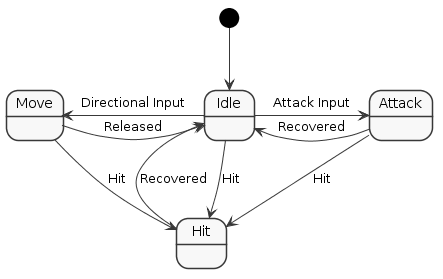
\includegraphics[width=\textwidth]{state.png}

\end{section}

\begin{section}{Moves}
Moves will be performed each frame by both characters. If an action input is
pressed, then the corresponding move will be performed. If a Left or Right input
is pressed, then the character will move left or right across the screen. If no
move is being inputted then the character will perform an idle move.

Each move will have a corresponding hitbox and hurtbox. If the hitbox from
one character's move overlaps with the hurtbox from the opposing character's
move, then the move is considered a hit.

The once exception is when the player being hit is moving away from the
attacking player. In this case, the hit is considered blocked instead.
\end{section}

\begin{section}{Move Statistics}
Moves will have three statistics: knock up, knock back, and damage. All three
values are constant for a given move, although they will vary from move to
move.

Knock up determines the upwards velocity given to the opponent when a move hits.
Larger knock up values will cause the opponent to be thrown higher into the air
when a hit is landed. Knock up is completely ignored upon a block.

Knock back determines how far away from the attacker the character being hit is
moved upon the completion of a successful hit. In addition to displacing by the
full knock back distance upon a hit, the character being attacked is displaced
one quarter of the distance if the hit is blocked instead.

Damage determines how much health is removed from the character being attacked.
In addition to removing the full damage amount from health on a successful hit,
one tenth of the damage will be removed from the target's health on a block.
\end{section}

\begin{section}{Move List}
Each character has five moves: idle, light attack, heavy attack, grab, and
special attack.

The most basic move is the idle move. This move has no hitbox and is the default
move in frames where no other move is being used.

The light attack move has the smallest knock up and knock back values, and the second smallest damage value of all a character's attacks. To compensate for
this, this move takes the fewest frames to complete, and has the fewest start up
frames (frames after the move is started but before there is a hitbox present)
and recovery frames (frames after the hitbox disappears but before the move is
finished).

The heavy attack has more knock up, knock back, and damage than the light
attack. In exchange, it has more start up frames and recovery frames than the
light attack.

The grab has the most knock up but a rather small knock back value. Furthermore,
it does not do much damage. Grabs come out very quickly, but have a very long
recovery.

Finally, there is the special attack. What this does varies from character to
character, but in each case this move does the most damage and has the longest
start up out of a character's moveset.
\end{section}

\chapter{Art}

Special thanks goes to Christian Boyd for helping me develop and sketch the
concept art for this game.

\begin{section}{Screens}
Sketches of the major screens present in the game.

\begin{subsection}{Main Menu}
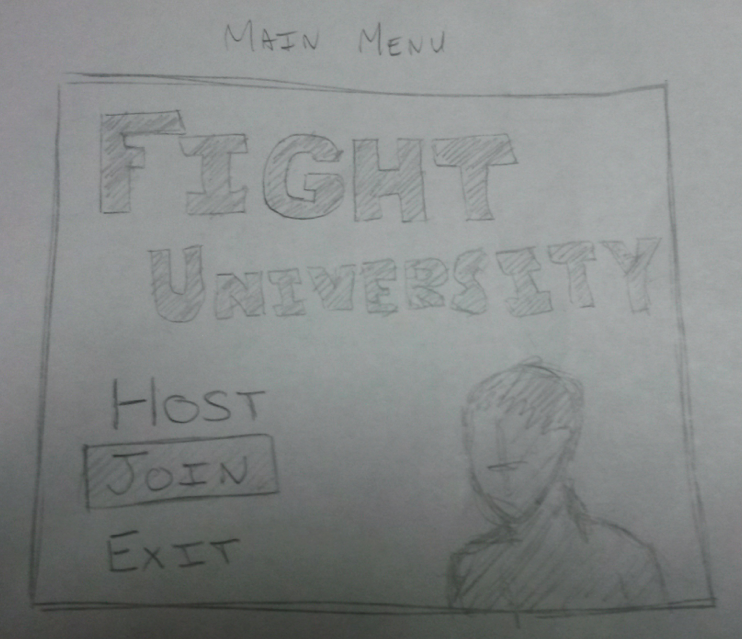
\includegraphics[width=\textwidth]{mainmenu.png}
\end{subsection}

\begin{subsection}{Character Selection}
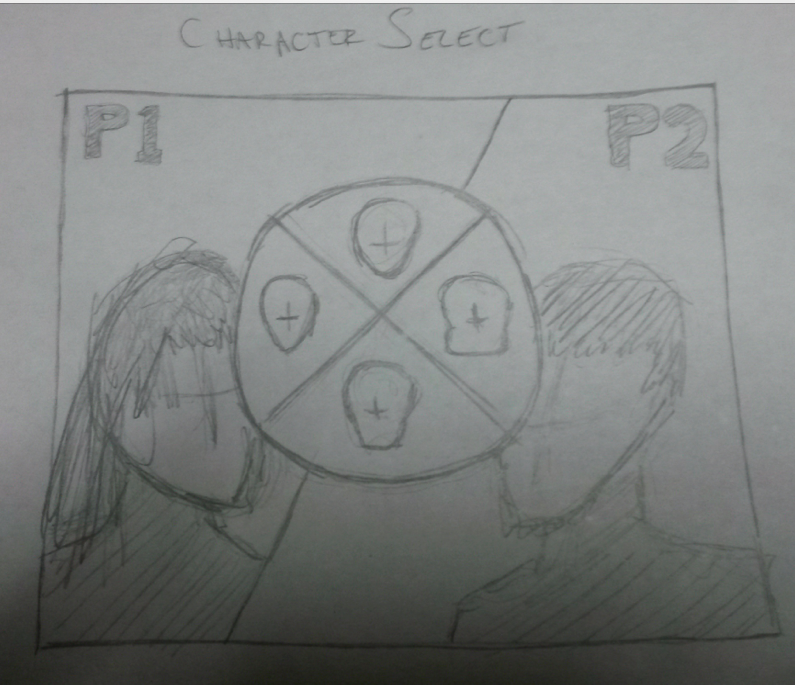
\includegraphics[width=\textwidth]{charselect.png}
\end{subsection}

\begin{subsection}{Combat}
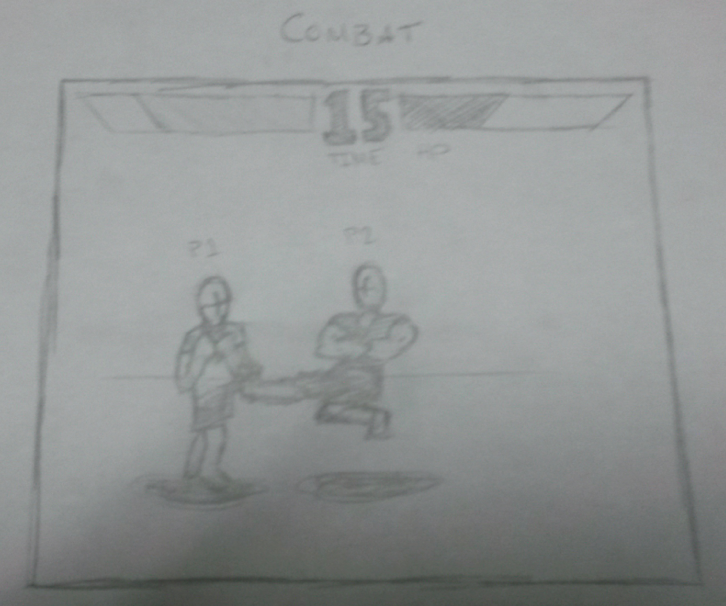
\includegraphics[width=\textwidth]{combat.png}
\end{subsection}

\end{section}

\begin{section}{Cast}
This game will feature four playable characters, each from a different major
offered at the fictional university.

\clearpage

\begin{subsection}{Chemistry}
The chemistry major is a fast, nimble character who fights at range by throwing
laboratory flasks. She is hard to catch, but doesn't do huge amounts of damage.

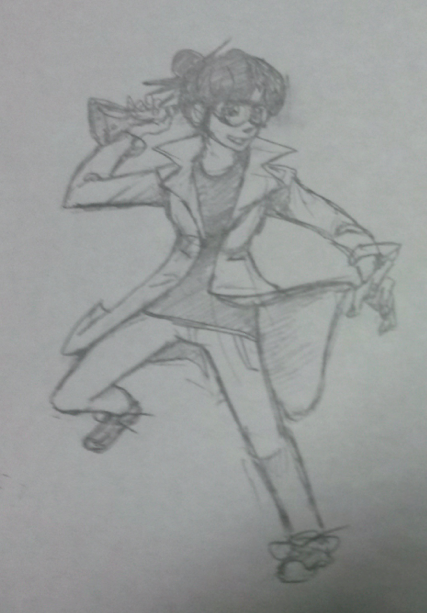
\includegraphics[height=8in]{chemistry.png}

\end{subsection}
\clearpage

\begin{subsection}{Business}
The business major is a slow, lumbering character who weilds a breifcase full
of documents. While most characters are faster, few can match his raw damage.

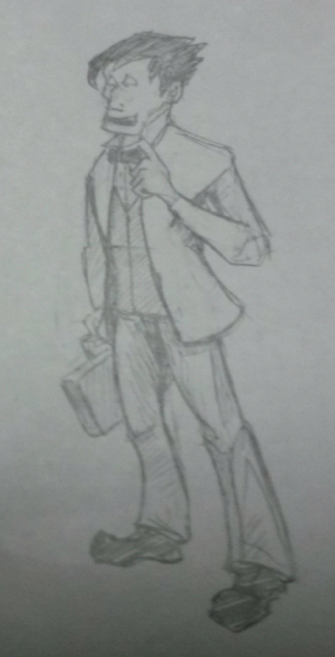
\includegraphics[height=8in]{business.png}

\end{subsection}
\clearpage

\begin{subsection}{Computer Science}
The computer science major is a more average character with a keyboard as his
weapon of choice. Damage is only average, but his special attack is to be
feared.

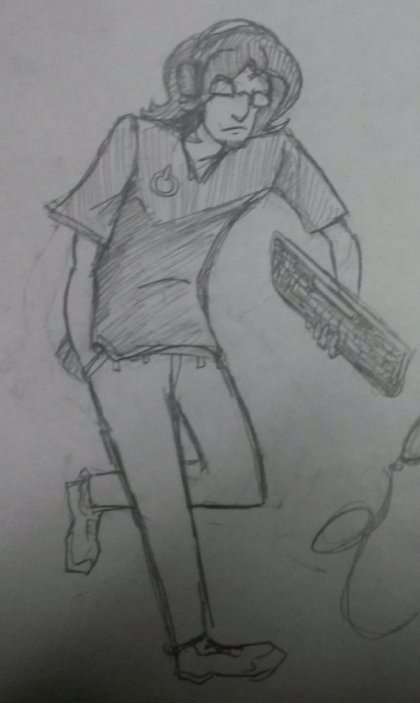
\includegraphics[height=8in]{compsci.png}

\end{subsection}
\clearpage

\begin{subsection}{Professor}
The professor uses a red pen and the threat of a bad grade to fight. While his
damage doesn't keep up with some of the other characters, his grabs are by far
the most effective.

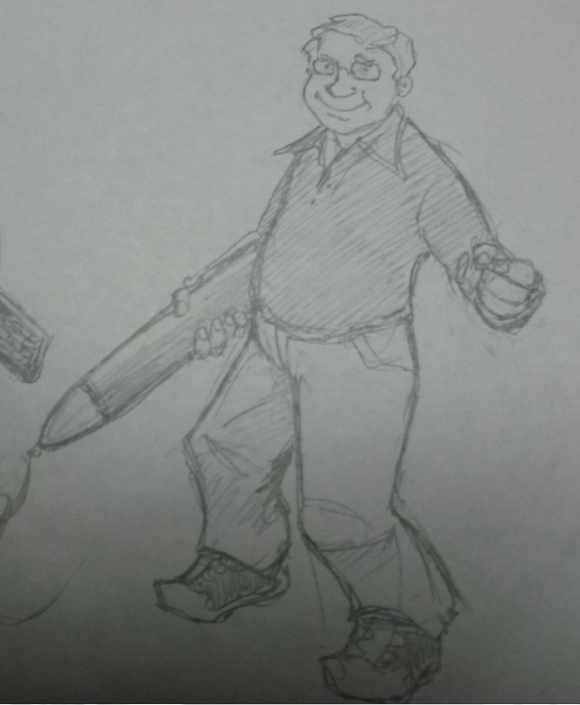
\includegraphics[height=8in]{professor.png}

\end{subsection}
\clearpage

\end{section}

\end{document}
